% ===================================================================== RESULTS
% Written after the last session (planned 9 Nov). One subsection per research question: state
% what the tables and figures show with \val{} numbers, then the pre-registered decision.
% Interpretation goes to the Discussion. Results stay preliminary until all
% \val{sessions-planned} sessions are in (the generated captions say so automatically).
% Macros available (see paper/generated/numbers.tex for the full list):
%  general  n-cases, sessions-done, gap-mean-pp, gap-min-pp, gap-max-pp, gap-fez-pp,
%           gap-kingston-pp, gap-twocurves-pp, gap-breastcancer-pp, gap-M1-pp ... gap-M3-pp
%  RQ1      h1-mean/lo/hi/decision, h1-slope, emu-over-count, emu-cases, emu-hw-r,
%           acc-EMU-<dataset>-<model>, acc-R0-..., acc-SIM-...
%  RQ2      h2-mean/lo/hi/decision, od-fez, od-kingston, od-M1..M3, od-frac-above-1,
%           r0-spread-mean-pp, r0-spread-max-pp, h4-decision, h4-largest, reg-largest,
%           reg-<term>-coef/lo/hi/p with term in readout, twoq, t1us, t2us, ageh
%  RQ3      nm-gamma-median/q1/q3, nm-absbeta-median, nm-r2-median/q1/q3, nm-gamma-M1..M3,
%           nm-r2-M1..M3, nm-gamma-sd-median, nm-fits
%  RQ4      gain-<method>-pp/lo/hi (methods R1, R28, R216, R232, R216s1, R3m, R3r, R4),
%           cost-<method>, gapshare-<method>, rep-best, rep-best-gain-pp, n-gap-cases,
%           h3-mean/lo/hi/decision, ece-<method>, brier-<method>, cov-<method>(-later/-min),
%           size-<method> (CPsim, CPs1, CPsame, ACI), h5-cps1-mean/lo/hi, h5-aci-mean/lo/hi,
%           h5-decision
\section{Results}
\label{sec:results}

% Simulator accuracy and classical baselines first (Table~\ref{tab:sim}).
\todo{Simulator results and baselines (Table~\ref{tab:sim}).}

% RQ1: Table~\ref{tab:accuracy} and Fig.~\ref{fig:emu-vs-hw}.
\subsection{Simulator, emulator and hardware (RQ1)}
\todo{RQ1.}

% RQ2: Fig.~\ref{fig:drift}; H2 and H4.
\subsection{Drift across sessions and devices (RQ2)}
\todo{RQ2.}

% RQ3: Fig.~\ref{fig:noise-model}.
\subsection{Noise model on Heron (RQ3)}
\todo{RQ3.}

% RQ4: Table~\ref{tab:repairs}, Fig.~\ref{fig:repair-cost}, Table~\ref{tab:coverage},
% Fig.~\ref{fig:coverage}; H3 and H5. Close with Table~\ref{tab:hypotheses}.
\subsection{Repairs and their cost (RQ4)}
\todo{RQ4.}

\begin{table*}[t]
\centering
\caption{Test accuracy by method, averaged over sessions and devices. SIM: noiseless simulator; EMU: calibration emulator; R0: hardware without repair; bold: best repair per row.}
\label{tab:accuracy}
\footnotesize
\setlength{\tabcolsep}{3.5pt}
\begin{tabular}{llccccccccc}
\toprule
Dataset & Model & SIM & EMU & R0 & R1 & R2$_{16}$ & R2$_{16}^{\mathrm{s1}}$ & R3$_{\mathrm{m}}$ & R3$_{\mathrm{r}}$ & R4 \\
\midrule
Breast cancer & M1 & 0.967 & 0.955 & 0.919 & 0.919 & 0.919 & 0.919 & \textbf{0.920} & 0.913 & 0.918 \\
Breast cancer & M2 & 0.933 & 0.915 & 0.921 & 0.923 & 0.921 & 0.922 & \textbf{0.925} & 0.921 & \textbf{0.925} \\
Breast cancer & M3 & 0.913 & 0.896 & 0.860 & 0.847 & 0.856 & 0.855 & \textbf{0.868} & 0.854 & 0.849 \\
Two curves & M1 & 0.927 & 0.903 & 0.829 & 0.826 & 0.829 & 0.830 & \textbf{0.841} & 0.824 & 0.825 \\
Two curves & M2 & 0.873 & 0.790 & 0.716 & 0.702 & 0.727 & 0.730 & 0.731 & 0.712 & \textbf{0.741} \\
Two curves & M3 & 0.847 & 0.781 & 0.663 & 0.685 & 0.676 & 0.669 & 0.683 & 0.676 & \textbf{0.701} \\
\bottomrule
\end{tabular}
\end{table*}

\begin{table}[t]
\centering
\caption{Repairs ranked by mean accuracy gain over R0 in percentage points, with a 95\% bootstrap interval over 60 cases (device, session, dataset, model); mean share of the simulator-to-hardware gap recovered in the 50 cases with a gap above 2 points; and extra QPU seconds per session.}
\label{tab:repairs}
\footnotesize
\setlength{\tabcolsep}{3.5pt}
\begin{tabular}{lccr}
\toprule
Repair & Gain (pp) & Gap (\%) & QPU (s) \\
\midrule
R3$_{\mathrm{m}}$ & +1.0 [+0.6, +1.5] & 15 & 1.06 \\
R4 & +0.8 [+0.2, +1.5] & 6 & 0.00 \\
R2$_{16}$ & +0.3 [+0.0, +0.7] & 3 & 0.25 \\
R2$_{16}^{\mathrm{s1}}$ & +0.3 [-0.1, +0.7] & 5 & 0.05 \\
R2$_{8}$ & +0.1 [-0.3, +0.4] & -0 & 0.13 \\
R1 & -0.1 [-0.6, +0.5] & -2 & 0.00 \\
R3$_{\mathrm{r}}$ & -0.1 [-0.7, +0.5] & -3 & 0.00 \\
R2$_{32}$ & -0.2 [-0.5, +0.1] & 1 & 0.50 \\
\bottomrule
\end{tabular}
\end{table}

\begin{table}[t]
\centering
\caption{Conformal prediction on hardware (target coverage 0.90): mean coverage over all sessions and over sessions 2 onward, worst case, mean set size and extra QPU seconds.}
\label{tab:coverage}
\footnotesize
\setlength{\tabcolsep}{3.5pt}
\begin{tabular}{lrrrrr}
\toprule
Method & Cov. & Cov.\ $s\geq2$ & Min & Size & QPU (s) \\
\midrule
CP$_{\mathrm{sim}}$ & 0.835 & 0.848 & 0.693 & 1.08 & 0.00 \\
CP$_{\mathrm{s1}}$ & 0.931 & 0.932 & 0.860 & 1.43 & 0.25 \\
CP$_{\mathrm{same}}$ & 0.919 & 0.909 & 0.793 & 1.38 & 0.50 \\
ACI & 0.899 & 0.908 & 0.880 & 1.30 & 0.00 \\
\bottomrule
\end{tabular}
\end{table}

\begin{table*}[t]
\centering
\caption{Pre-registered hypotheses, test statistics (mean and 95\% bootstrap interval) and decisions. Preliminary: 2 of 10 sessions.}
\label{tab:hypotheses}
\footnotesize
\setlength{\tabcolsep}{3.5pt}
\begin{tabular}{llll}
\toprule
 & Hypothesis & Statistic & Decision \\
\midrule
H1 & Emulator overestimates hardware accuracy & EMU$-$R0 0.074 [0.044, 0.105] & supported \\
H2 & Session-to-session variation exceeds shot noise & -- & pending \\
H3 & Refit on 16 labels (R2$_{16}$) beats normalisation (R1) & R2$_{16}-$R1 0.013 [-0.001, 0.029] & not supported \\
H4 & Readout error is the strongest calibration predictor & largest: age\_h & not supported \\
H5 & Split CP under-covers later sessions; ACI holds & -- & pending \\
\bottomrule
\end{tabular}
\end{table*}


% Fig. 1 of results/figures (simulator vs emulator vs hardware bars) repeats Table IV and is
% left out of the paper to stay within 8 pages.

\begin{figure}[t]
\centering
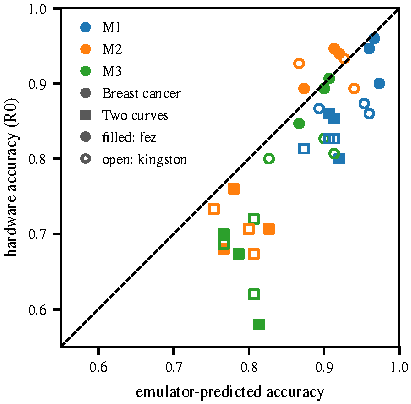
\includegraphics[width=\columnwidth]{fig3_emulator_vs_hardware.pdf}
\caption{Emulator-predicted against hardware accuracy (R0). Each point is one session, dataset
and model; colour marks the model, shape the dataset, and filled or open markers the device.
The dashed line marks equality.}
\label{fig:emu-vs-hw}
\end{figure}

\begin{figure*}[t]
\centering
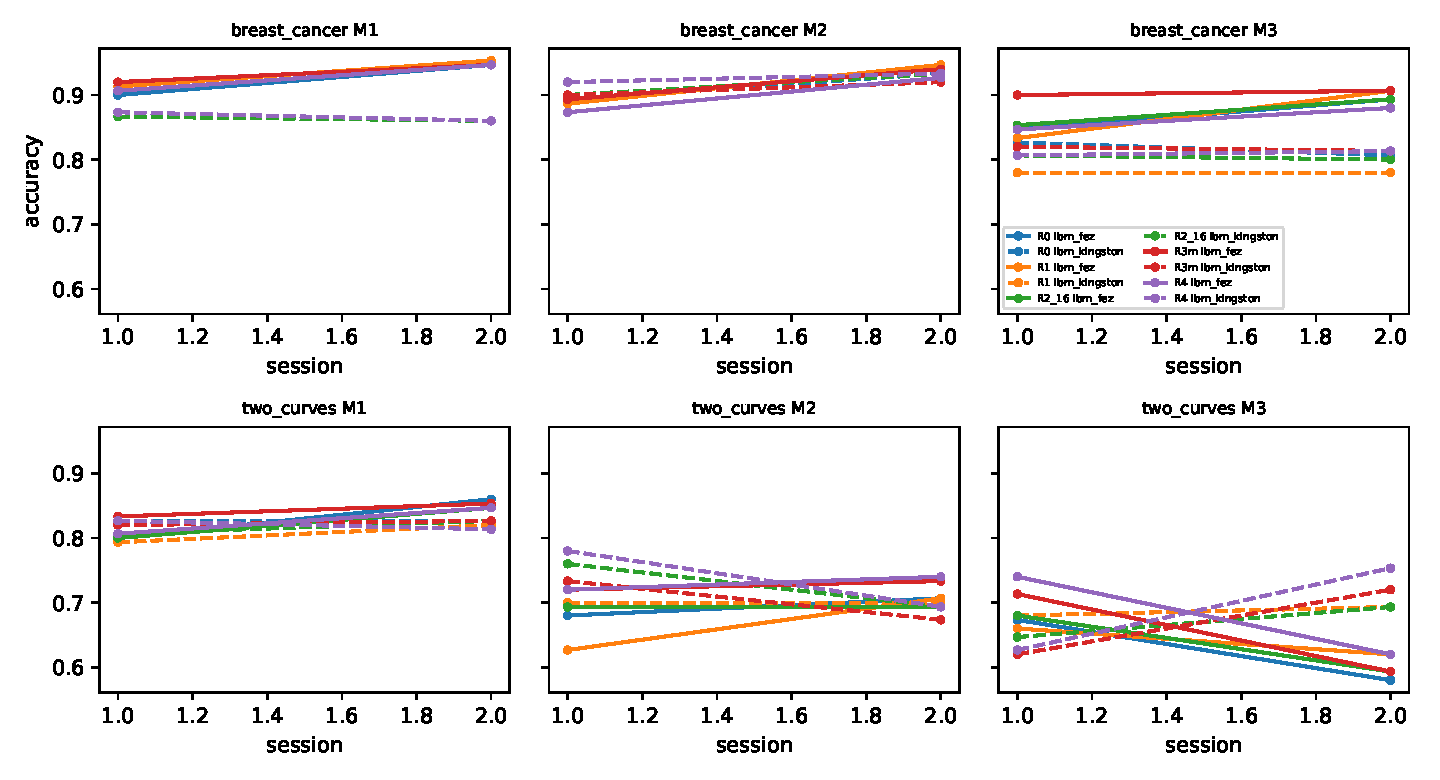
\includegraphics[width=\textwidth]{fig2_drift.pdf}
\caption{Hardware test accuracy per session for each dataset and model: R0 with 95\% bootstrap
intervals and selected repairs; solid and dashed lines are the two devices, and the dotted grey
line is the noiseless simulator.}
\label{fig:drift}
\end{figure*}

\begin{figure}[t]
\centering
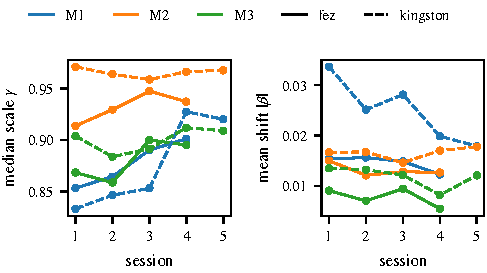
\includegraphics[width=\columnwidth]{fig4_noise_model.pdf}
\caption{Linear map from simulator to hardware features, $\phi_{\mathrm{hw}}\approx\gamma\,
\phi_{\mathrm{sim}}+\beta$, fitted per feature and session: median scale and mean absolute
shift by model and device.}
\label{fig:noise-model}
\end{figure}

\begin{figure}[t]
\centering
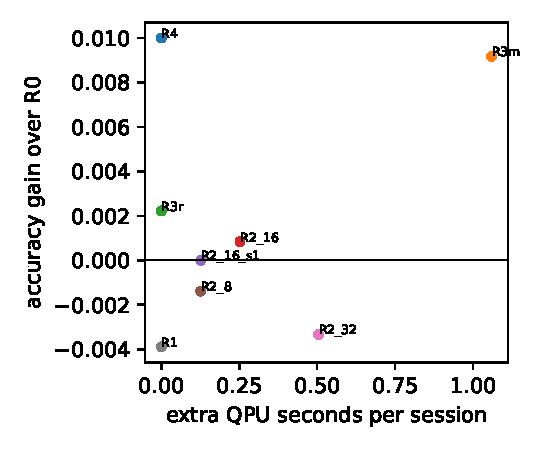
\includegraphics[width=\columnwidth]{fig5_repair_cost.pdf}
\caption{Mean accuracy gain of each repair over R0, with 95\% bootstrap intervals, against the
extra QPU seconds it needs per session. Repairs with equal cost are spread horizontally for
readability.}
\label{fig:repair-cost}
\end{figure}

\begin{figure}[t]
\centering
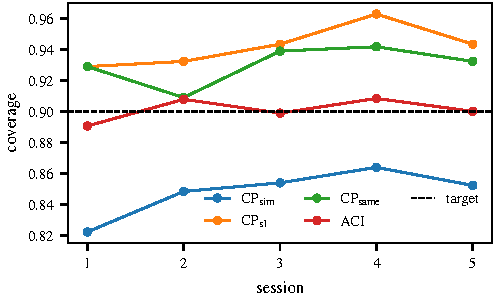
\includegraphics[width=\columnwidth]{fig6_coverage.pdf}
\caption{Conformal coverage per session, averaged over devices, datasets and models; the dashed
line is the target \val{coverage-target}.}
\label{fig:coverage}
\end{figure}
